\chapter{Estado da Arte}

% [NOTA: Adicionar citações bibliográficas em todo o capítulo]

\section{Sistemas de Gestão Medicamentosa Hospitalar}

\subsection{Evolução Histórica}

Os sistemas de informação hospitalar (HIS) evoluíram significativamente desde os primeiros sistemas baseados em mainframes dos anos 1960. A transição para sistemas departamentais nos anos 1980 e a posterior integração através de Health Level Seven (HL7) \cite{dolin2006,mandl2020} nos anos 1990 estabeleceram as bases para os sistemas modernos.

\begin{figure}[htbp]
    \centering
    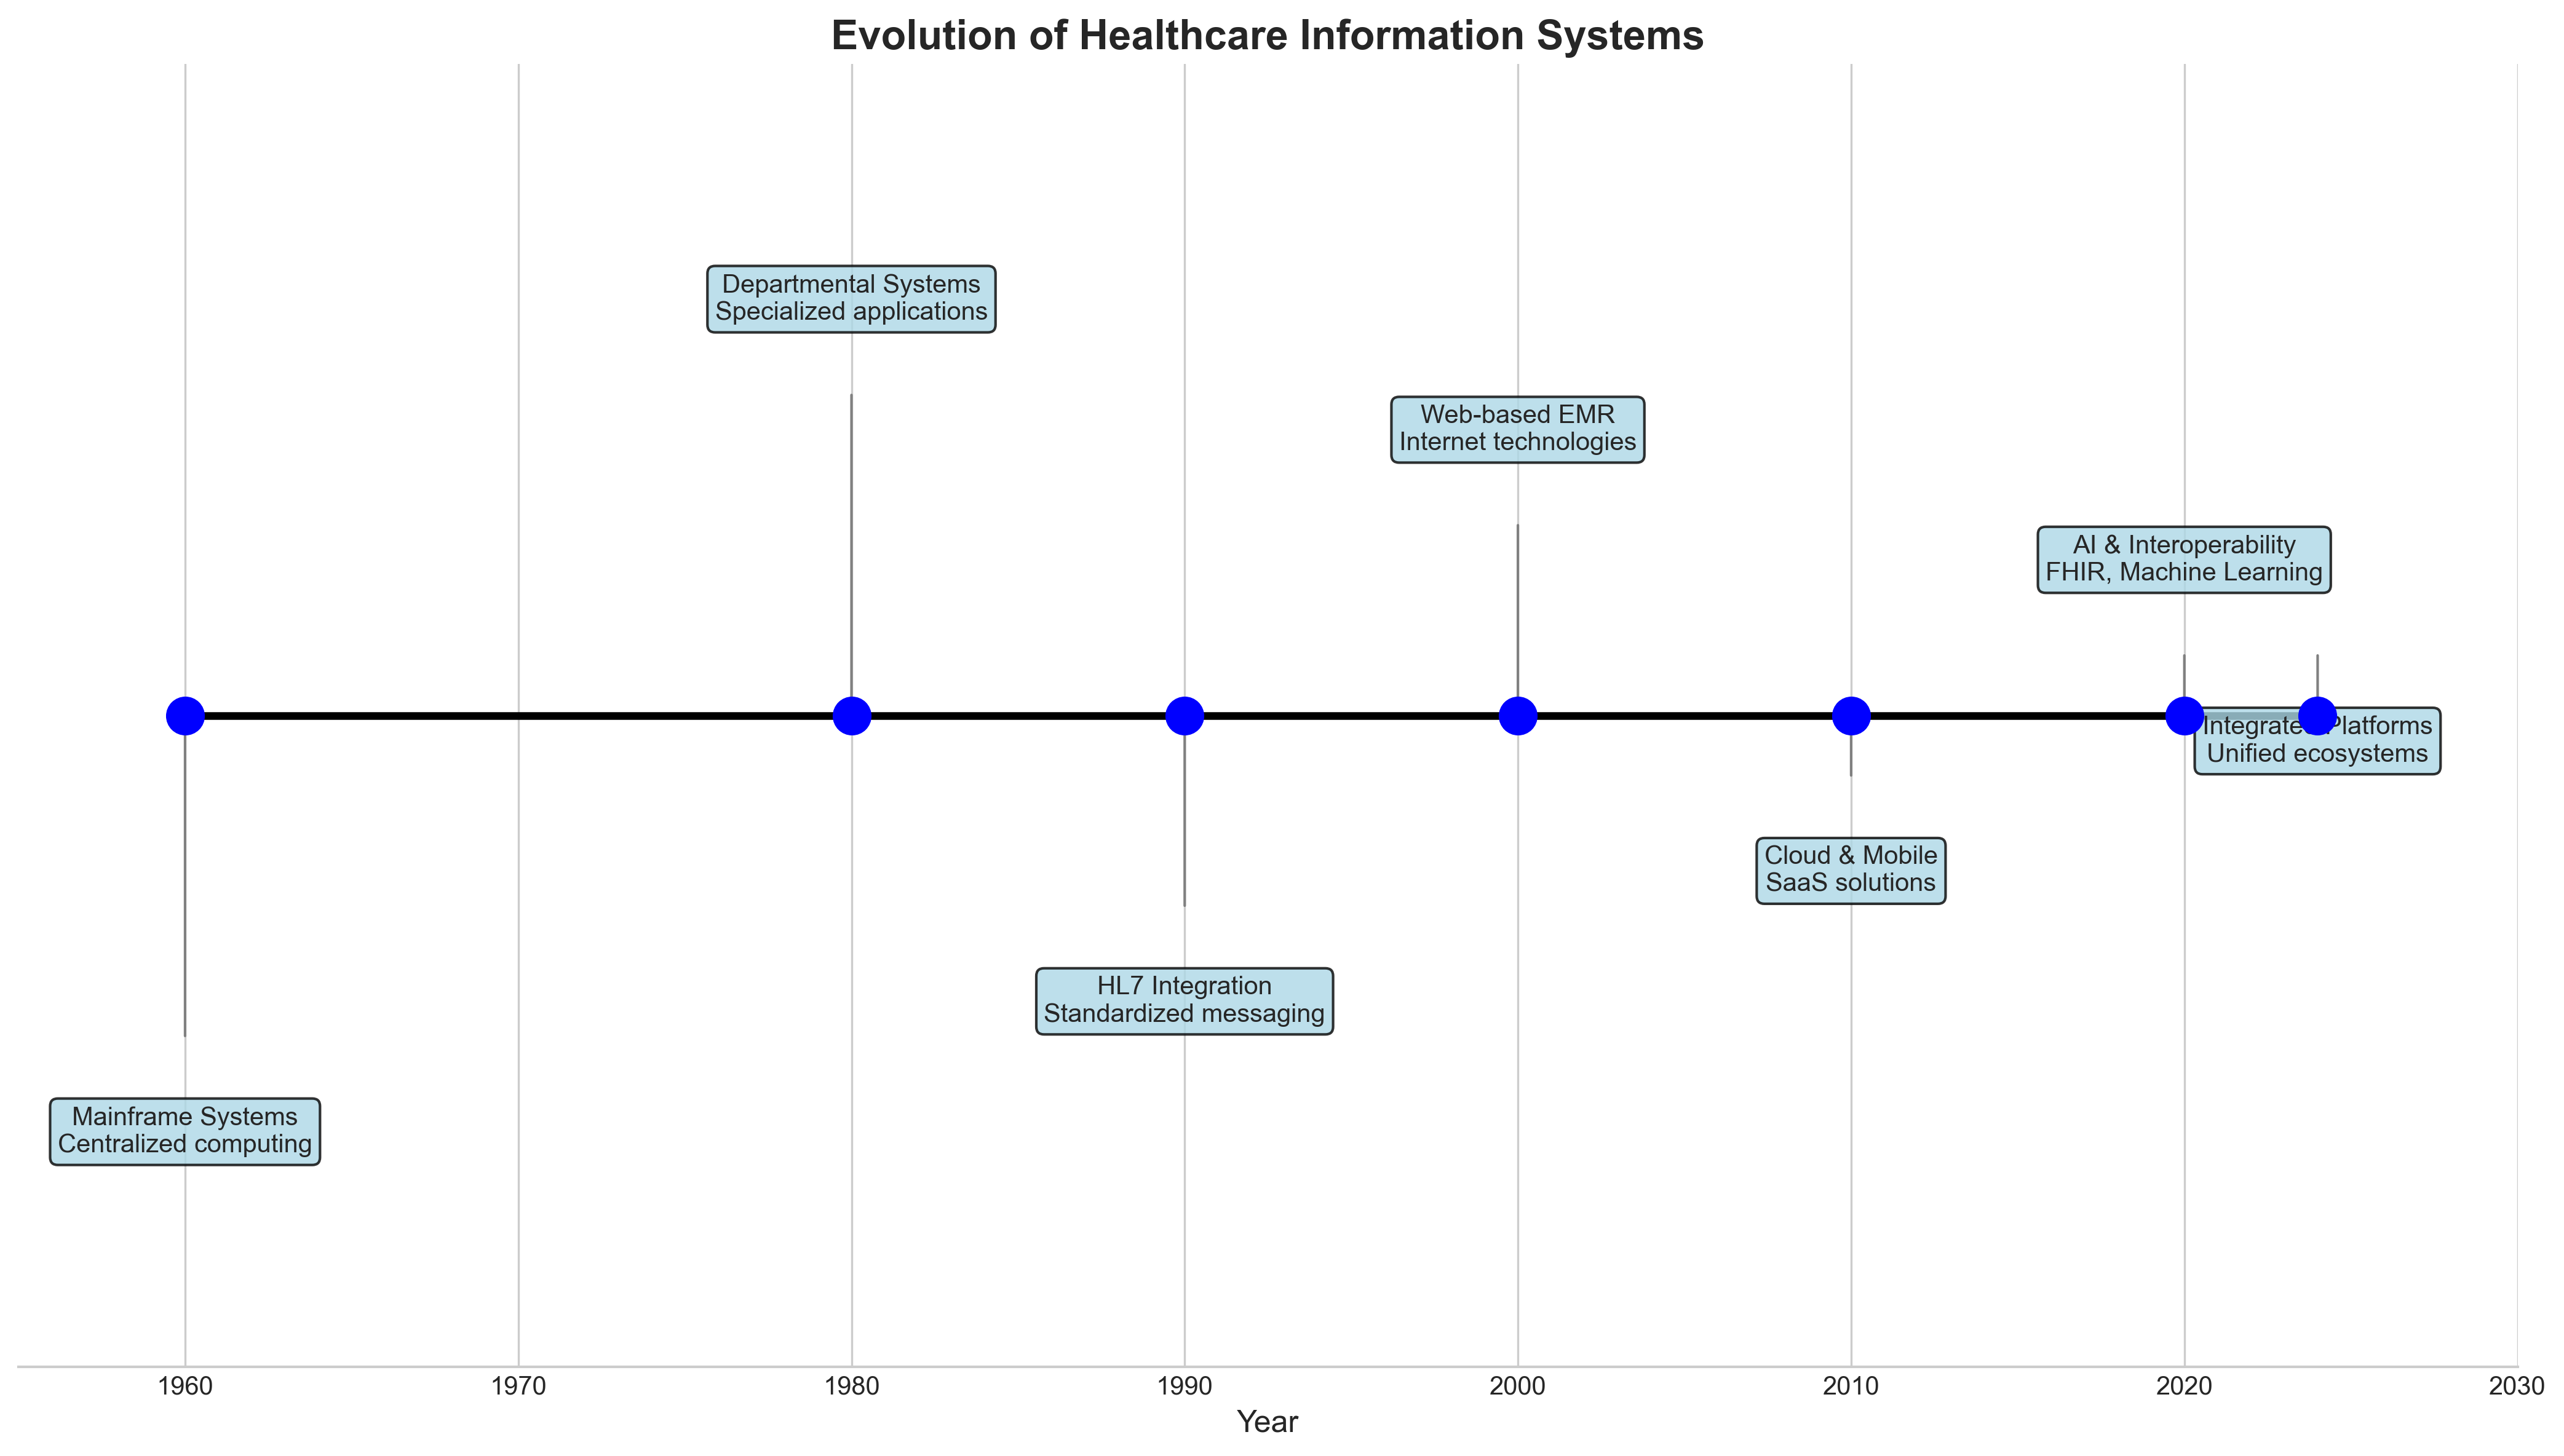
\includegraphics[width=0.95\textwidth]{images/generated/healthcare_it_timeline.png}
    \caption{Evolution of healthcare information systems from mainframe to integrated platforms \citep{shermock2023,vaghasiya2023}.}
    \label{fig:timeline}
\end{figure}

\subsection{Sistemas Comerciais Atuais}

O panorama atual dos sistemas comerciais de gestão hospitalar é dominado por alguns fornecedores principais. A Epic Systems \cite{hertzum2022} estabeleceu-se como líder de mercado nos Estados Unidos com o seu sistema EpicCare, oferecendo uma plataforma integrada para gestão clínica e administrativa. A Cerner, recentemente adquirida pela Oracle Health \cite{lin2018}, compete diretamente com as suas soluções PowerChart e Millennium, particularmente populares em hospitais de média e grande dimensão.

No mercado europeu, destaca-se a InterSystems com o TrakCare, que ganhou aceitação significativa devido à sua capacidade de adaptação a diferentes contextos regulamentares. A Allscripts, com o Sunrise Clinical Manager, mantém uma posição relevante especialmente em hospitais que procuram soluções mais flexíveis e personalizáveis.

% [INSERIR: Tabela 2.1 - Comparação de funcionalidades dos principais sistemas]

\subsection{Desafios dos Sistemas Atuais}

Apesar dos avanços tecnológicos, os sistemas atuais enfrentam desafios significativos que limitam a sua eficácia. A interoperabilidade limitada \cite{keasberry2017} representa um obstáculo major, com a falta de standards efetivos a impedir a comunicação seamless entre diferentes sistemas hospitalares. Esta fragmentação resulta em silos de informação que comprometem a continuidade de cuidados.

A complexidade das interfaces \cite{mcgreevey2020} constitui outro desafio crítico, frequentemente causando fadiga de alertas nos profissionais de saúde. Os custos elevados \cite{adler2021} de implementação e manutenção representam uma barreira significativa, especialmente para hospitais de menor dimensão. Finalmente, a resistência à mudança \cite{holden2011,venkatesh2003} permanece um fator limitante, refletindo a importância dos fatores humanos e organizacionais na adoção de novas tecnologias.

\section{Segurança na Medicação}

% [DESENVOLVER: Adicionar estatísticas europeias e nacionais]

Os erros de medicação \cite{ciapponi2021,mulac2020} constituem uma das principais causas de eventos adversos evitáveis:
- Globalmente: 1 em 10 pacientes afetados (OMS, 2022)
- Europa: 8-12\% das admissões hospitalares % [CITAR: European Commission Report \cite{european2016}]
- Portugal: Dados limitados mas estimativas similares \cite{dgs2020} % [CONTACTAR: DGS para dados oficiais]

\subsection{Tipos de Erros Mais Frequentes}

\begin{enumerate}
    \item \textbf{Erros de prescrição} (30-40\%): Dose incorreta, medicamento errado \cite{isaacs2021}
    \item \textbf{Erros de transcrição} (12-20\%): Interpretação incorreta \cite{manias2021}
    \item \textbf{Erros de dispensa} (11-15\%): Troca de medicamentos \cite{kallio2020}
    \item \textbf{Erros de administração} (26-38\%): Via, horário ou paciente errado \cite{boytim2018}
\end{enumerate}

\begin{figure}[htbp]
    \centering
    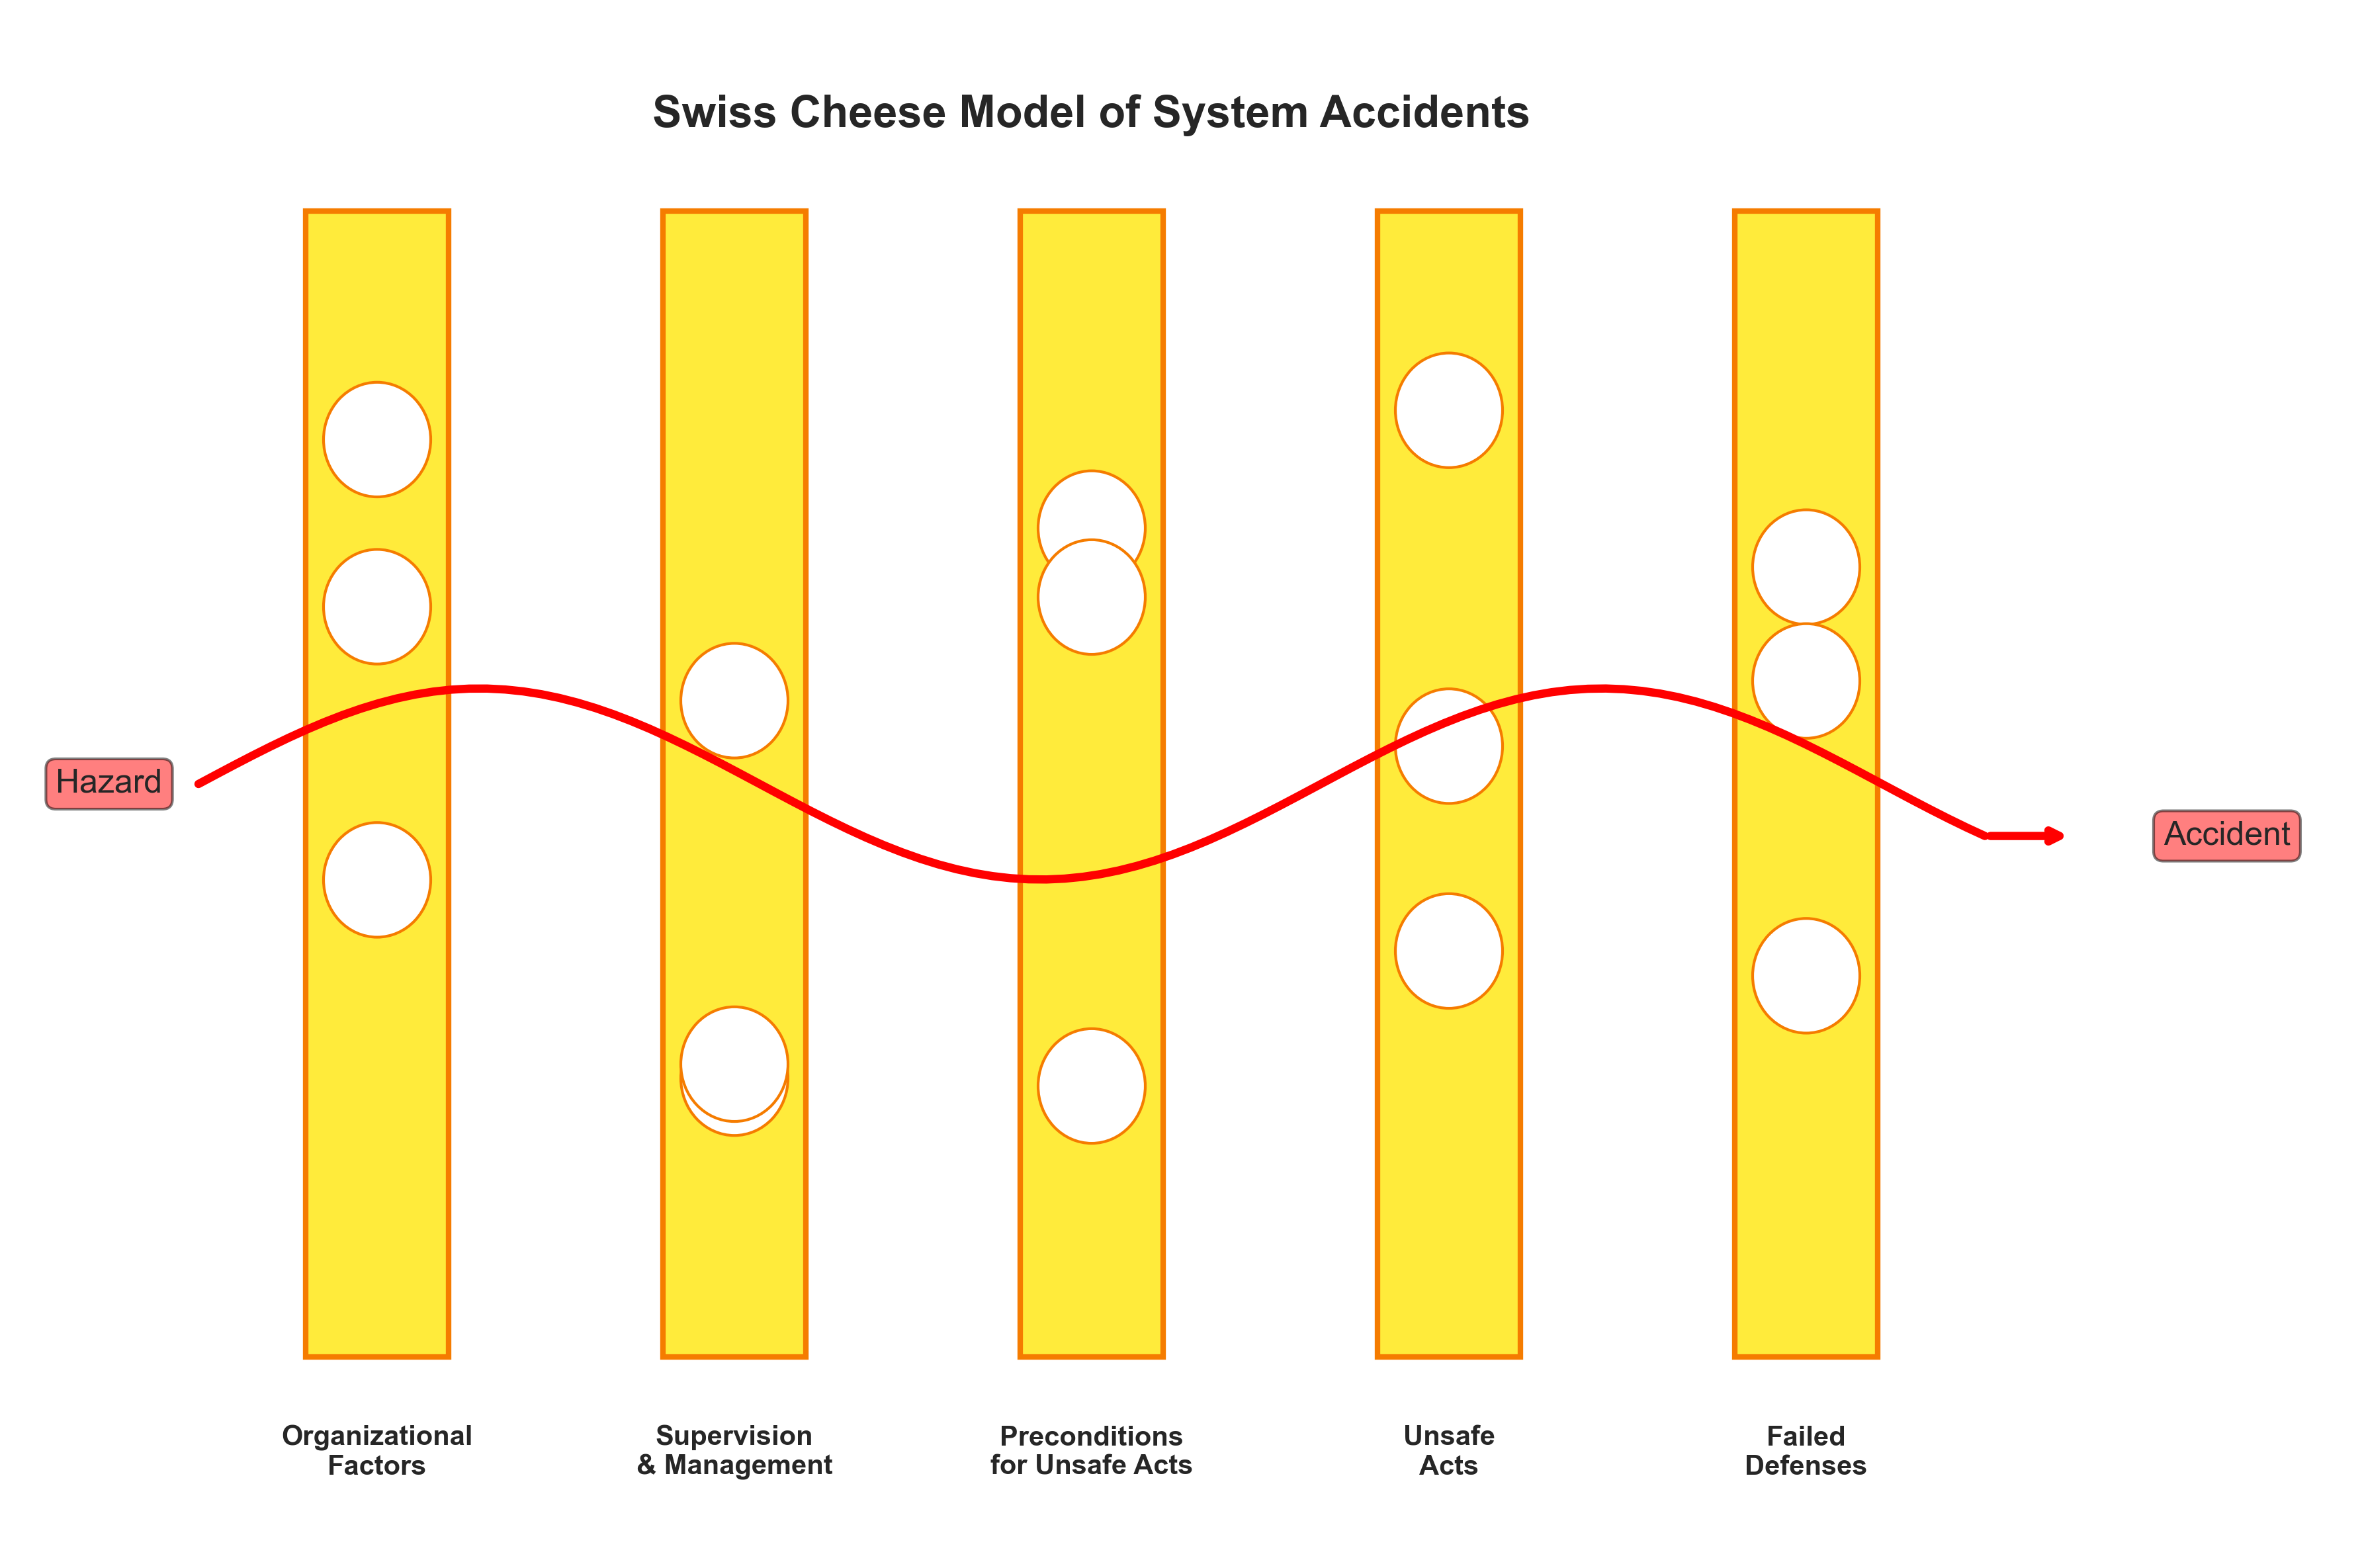
\includegraphics[width=0.85\textwidth]{images/generated/swiss_cheese_model.png}
    \caption{Swiss Cheese Model applied to medication errors showing how system failures align to cause accidents. Based on Reason's model \citep{ciapponi2021,mulac2020}.}
    \label{fig:swiss_cheese}
\end{figure}

\section{Tecnologias Emergentes}

\subsection{Clinical Decision Support Systems (CDSS)}

Os sistemas de apoio à decisão clínica \cite{moss2015,belle2013} representam uma categoria fundamental de ferramentas tecnológicas em saúde:

Os CDSS modernos integram:
- Verificação de interações em tempo real
- Alertas baseados em guidelines
- Machine learning \cite{bates2021,zhao2021} para personalização

% [CITAR: Estudos de eficácia - Bright et al., 2022 \cite{amland2019}; Kwan et al., 2023]

\subsection{Inteligência Artificial em Saúde}

\subsubsection{Natural Language Processing}

A aplicação de processamento de linguagem natural \cite{rozenblum2020} em sistemas de gestão medicamentosa permite:
- BioBERT e ClinicalBERT para extração de informação % [CITAR: Lee et al., 2020]
- Deteção automática de eventos adversos % [CITAR: Wang et al., 2021]

\subsubsection{Machine Learning}
- Previsão de readmissões
- Otimização de doses
- Identificação de padrões de prescrição

% [INSERIR: Tabela 2.2 - Aplicações de IA em gestão medicamentosa]

\subsection{Blockchain em Saúde}
- Rastreabilidade de medicamentos \cite{franzoso2014}
- Gestão descentralizada de consentimentos
- Auditoria imutável de prescrições

\section{Arquiteturas e Tecnologias de Implementação}

\subsection{Arquiteturas de Microserviços}

% [NOTA: Mover conteúdo técnico repetido da metodologia para cá]

Vantagens para sistemas hospitalares \cite{shermock2023,vaghasiya2023}:
- Escalabilidade independente
- Resiliência a falhas
- Atualizações sem downtime \cite{greenhalgh2017}
- Integração facilitada com sistemas legados \cite{newman2021}

\subsection{Padrões de Integração}

\begin{itemize}
    \item \textbf{API Gateway}: Ponto único de entrada \cite{newman2021}
    \item \textbf{Service Mesh}: Comunicação entre serviços
    \item \textbf{Event-Driven}: Arquitetura assíncrona \cite{fowler2018}
    \item \textbf{CQRS}: Separação de comandos e queries
\end{itemize}

\section{Contexto Nacional}

Em Portugal, a digitalização da saúde tem avançado através de iniciativas como:
- PDS (Plataforma de Dados da Saúde) \cite{sns2019}
- RSE (Registo de Saúde Eletrónico)
- PEM (Prescrição Eletrónica de Medicamentos) \cite{dgs2020}

No entanto, persistem desafios significativos:
- Fragmentação entre sistemas hospitalares
- Falta de interoperabilidade entre regiões \cite{keasberry2017}
- Resistência à mudança por parte dos profissionais \cite{venkatesh2003}
- Investimento limitado em modernização tecnológica

\begin{figure}[htbp]
    \centering
    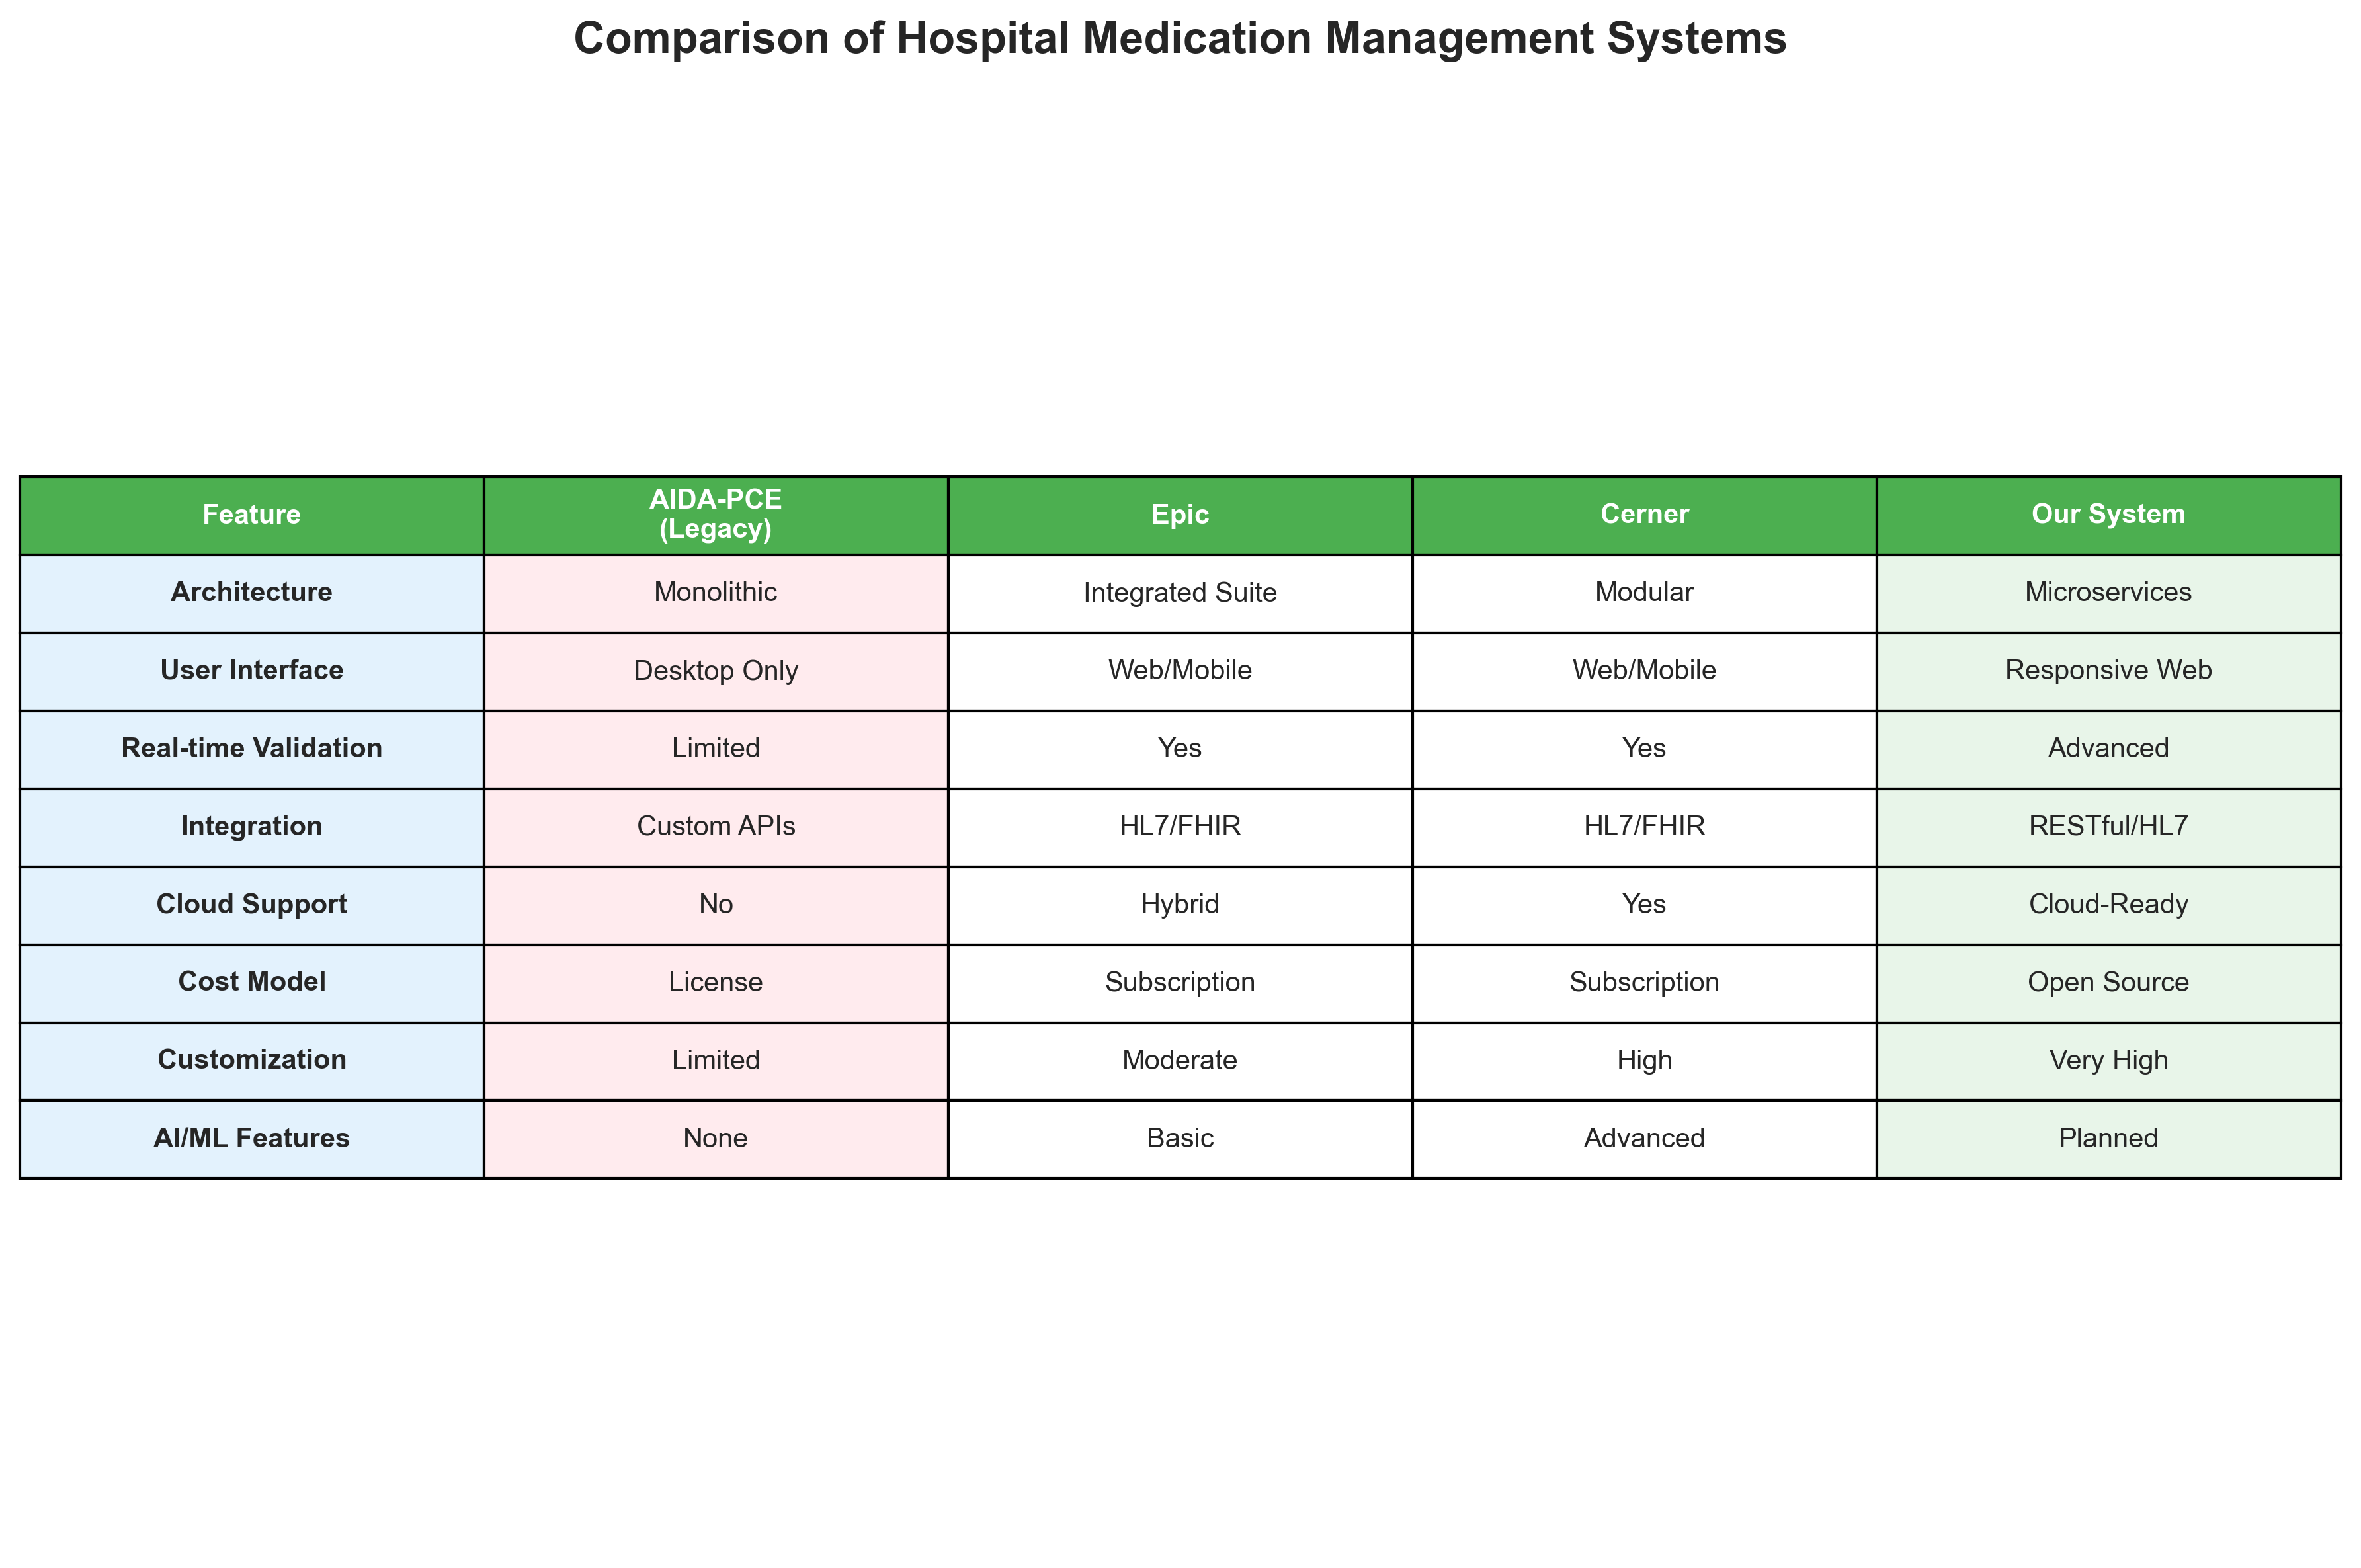
\includegraphics[width=0.95\textwidth]{images/generated/system_comparison_table.png}
    \caption{Comparative analysis of hospital medication management systems including legacy and modern solutions.}
    \label{tab:comparison}
\end{figure}

\section{Standards e Interoperabilidade}

\subsection{HL7 FHIR}

Fast Healthcare Interoperability Resources representa a evolução do HL7:
- APIs RESTful nativas
- Recursos modulares
- Suporte para aplicações móveis

% [INSERIR: Exemplo de recurso FHIR para prescrição]

\subsection{Standards Nacionais}

Em Portugal:
- PEM (Prescrição Eletrónica de Medicamentos)
- BDNP (Base de Dados Nacional de Prescrições)
- RNU (Registo Nacional de Utentes)

\section{Lacunas e Oportunidades}

\subsection{Lacunas Identificadas}

1. \textbf{Integração deficiente}: Silos de informação persistem
2. \textbf{Usabilidade}: Interfaces não otimizadas para workflow clínico
3. \textbf{Contexto nacional}: Soluções não adaptadas à realidade portuguesa
4. \textbf{Custo-benefício}: ROI difícil de demonstrar

\subsection{Oportunidades de Investigação}

Este trabalho endereça as lacunas através de:
- Arquitetura de integração não-invasiva
- Design centrado no utilizador
- Adaptação ao contexto português
- Modelo de implementação incremental

% [INSERIR: Figura 2.3 - Posicionamento da solução proposta no estado da arte]

\section{Síntese e Posicionamento do Trabalho}

% [NOTA: Remover redundâncias com a introdução]

A revisão da literatura revela que, apesar dos avanços tecnológicos, persiste uma lacuna entre as capacidades técnicas e a implementação efetiva em contextos reais. Este trabalho contribui com uma abordagem pragmática que equilibra inovação tecnológica com viabilidade de implementação no contexto específico do sistema de saúde português. 